\documentclass[11pt]{article}

% This is a package for drawing figures
% it is a part of standard latex 2e distribution
\usepackage{tikz}
\usetikzlibrary{shapes}
\usepackage{fullpage}


\usepackage{palatino}
\RequirePackage{ifthen}
\usepackage{latexsym}
\RequirePackage{amsmath}
\RequirePackage{amsthm}
\RequirePackage{amssymb}
\RequirePackage{xspace}
\RequirePackage{graphics}
\usepackage{xcolor}

\usepackage{stmaryrd}


\RequirePackage{textcomp}
\usepackage{keyval}
%\usepackage{listings}
\usepackage{xspace}
\usepackage{mathrsfs,paralist, amsmath,amssymb,url,listings,mathrsfs}
%\usepackage{pvs}
%\usepackage{supertabular,alltt,latexsym}
%\usepackage{multicol,multirow,epsfig}
%\usepackage[dvips, usenames]{color}
\usepackage{framed}
\usepackage{lipsum}
%\usepackage[dvipsnames]{color}

% copyright notice


\definecolor{reddish}{rgb}{1,.8,0.8}
\definecolor{blueish}{rgb}{0.8,.8,1}
\definecolor{greenish}{rgb}{.8,1,0.8}
\definecolor{yellowish}{rgb}{1,1,.20}


\usepackage[pdftex]{hyperref}
\hypersetup{
  pdftitle={Homework for Modeling and Verification of Real-time and Hybrid Systems},
  pdfauthor={Sayan Mitra},
  colorlinks=true,
  citecolor={blue},
  linkcolor = {blue},
  pagecolor={blue},
  backref={true},
  bookmarks=true,
  bookmarksopen=false,
  bookmarksnumbered=true
}

%\newcommand{\remove}[1]{}
\newcommand{\nicole}[1]{\textcolor{red}{#1}}

\newcommand{\handout}[6]{
  \noindent
  \begin{center}
  \framebox{
    \vbox{
      \hbox to 5.78in { {\bf ECE/CS 584: Embedded and cyberphysical system  verification } \hfill #2 }
      \vspace{4mm}
      \hbox to 5.78in { {\Large \hfill #5  \hfill} }
      \vspace{2mm}
       \hbox to 5.78in { {\Large \hfill #6  \hfill} }
      \vspace{2mm}
      \hbox to 5.78in { {\em #3 \hfill #4} }
    }
  }
  \end{center}
  \vspace*{4mm}
}

\newcommand{\smallheader}[5]{
  \noindent
  \begin{center}
  \framebox{
    \vbox{
      \hbox to 5.78in { {\bf ECE/CS 584: Embedded and cyberphysical system  verification  } \hfill #2 }
      \vspace{2mm}
      \hbox to 5.78in { {\em #3 \hfill #4} }
      \vspace{2mm}
      \hbox to 5.78in { {\em \hfill #5} }
    }
  }
  \end{center}
  \vspace*{4mm}
}

\newcommand{\lecture}[4]{\handout{#1}{#2}{#3}{Scribe: #4}{Lecture #1}}

\newcommand{\homework}[2]{\smallheader{#1}{Fall 2019}{Homework #1}\vspace{5mm}
	{#2}
	}

\newcommand{\solution}[2]{\smallheader{#1}{Fall 2017}{Solutions for Homework #1}{#2}}

\newcommand{\reals}[0]{\mathbb{R}}
\newcommand{\reach}[0]{Reach}
\newcommand{\A}[0]{\mathcal{A}}
\newcommand{\tab}{\hspace*{5mm}}

\newcommand{\interestingfact}[1]{
	\noindent
	\begin{center}
	\colorbox{yellowish}{
	\parbox{11.5cm}{{\bf Factoid.} #1}
	}
	\end{center}
	\vspace*{4mm}
}
%\definecolor{MyGray}{rgb}{0.96,0.97,0.98}
\makeatletter\newenvironment{color1box}{%
   \begin{lrbox}{\@tempboxa}\begin{minipage}{\columnwidth}}{\end{minipage}\end{lrbox}%
   \colorbox{reddish}{\usebox{\@tempboxa}}
}\makeatother


\makeatletter\newenvironment{color3box}{%
   \begin{lrbox}{\@tempboxa}\begin{minipage}{\columnwidth}}{\end{minipage}\end{lrbox}%
   \colorbox{blueish}{\usebox{\@tempboxa}}
}\makeatother

% 1-inch margins, from fullpage.sty by H.Partl, Version 2, Dec. 15, 1988.
\topmargin 0pt
\advance \topmargin by -\headheight
\advance \topmargin by -\headsep
\textheight 8.9in
\oddsidemargin 0pt
\evensidemargin \oddsidemargin
\marginparwidth 0.5in
\textwidth 6.5in

\parindent 0in
\parskip 1.5ex
%\renewcommand{\baselinestretch}{1.25}

\begin{document}


\smallheader{2 on Modeling physics and cyberphysicsl systems--- Due on October $3^{rd}$}{Fall 2019}{Dawei Sun, daweis2}{Homework 2: Modeling physics and cyberphysicsl systems}{Due October $3^{rd}$}

\begin{quote}
	{\em Typeset your solutions using \LaTeX\, zip your writeup (.pdf) and code (.py) in a single file called \texttt{nedid-584-F19.zip} and upload this file through Compass.}
\end{quote}

\paragraph{Problem 1. Convexity of reach sets (20 points)}
(a) For a linear autonomous system $\dot{x} = Ax$, $x \in \reals^n$, prove that if the set of initial states $\Theta$ is a polytope with a set of vertices $v_1, \ldots, v_k \in \reals^n$, then the set of reachable states at any time $t > 0$ is also a convex set. That is, $\reach{}(\Theta,t)$ is the convex hull of the points reached from the vertices of $\Theta$ at time $t$.

(b) Give an example of a nonlinear system for which $\reach{}(\Theta,t)$ is not convex, even if $\Theta$ is convex. You can give an analytical proof or a numerical example. You may consider a discrete time model $x(t+1) = f(x(t))$ as well.

\paragraph{Solution}
\begin{enumerate}[(a)]
\item
$\forall x^1, x^2 \in \reach{}(\Theta, t)$, denote $x_0^1, x_0^2$ as the corresponding initial state, then we have $x^1 = e^{At}x_0^1, x^2 = e^{At}x_0^2$, and thus $\forall \lambda \in [0,1]$ we have $\lambda x^1 + (1 - \lambda) x^2 = e^{At}(\lambda x_0^1 + (1 - \lambda)x_0^2)$. Because $\Theta$ is convex and $x_0^1, x_0^2 \in \Theta$, we have $(\lambda x_0^1 + (1 - \lambda)x_0^2) \in \Theta$, and thus $e^{At}(\lambda x_0^1 + (1 - \lambda)x_0^2) \in \reach{}(\Theta, t)$. Because $x^1, x^2$ are chosen arbitraily, we proved that $\reach{}(\Theta, t)$ is convex.
\item
Consider a two-dimensional non-linear discrete time system.
$$x(t+1) = \begin{cases}
      0, & \text{if}~x(t)_1 > 0, x(t)_2 > 0\\
      x(t), & \text{otherwise}\\
    \end{cases}
$$

As shown in Fig. \ref{fig:convex} starting from a convex set $\Theta$, $\reach{}(\Theta, t)$ is not convex.

\begin{figure}[h]
\centering
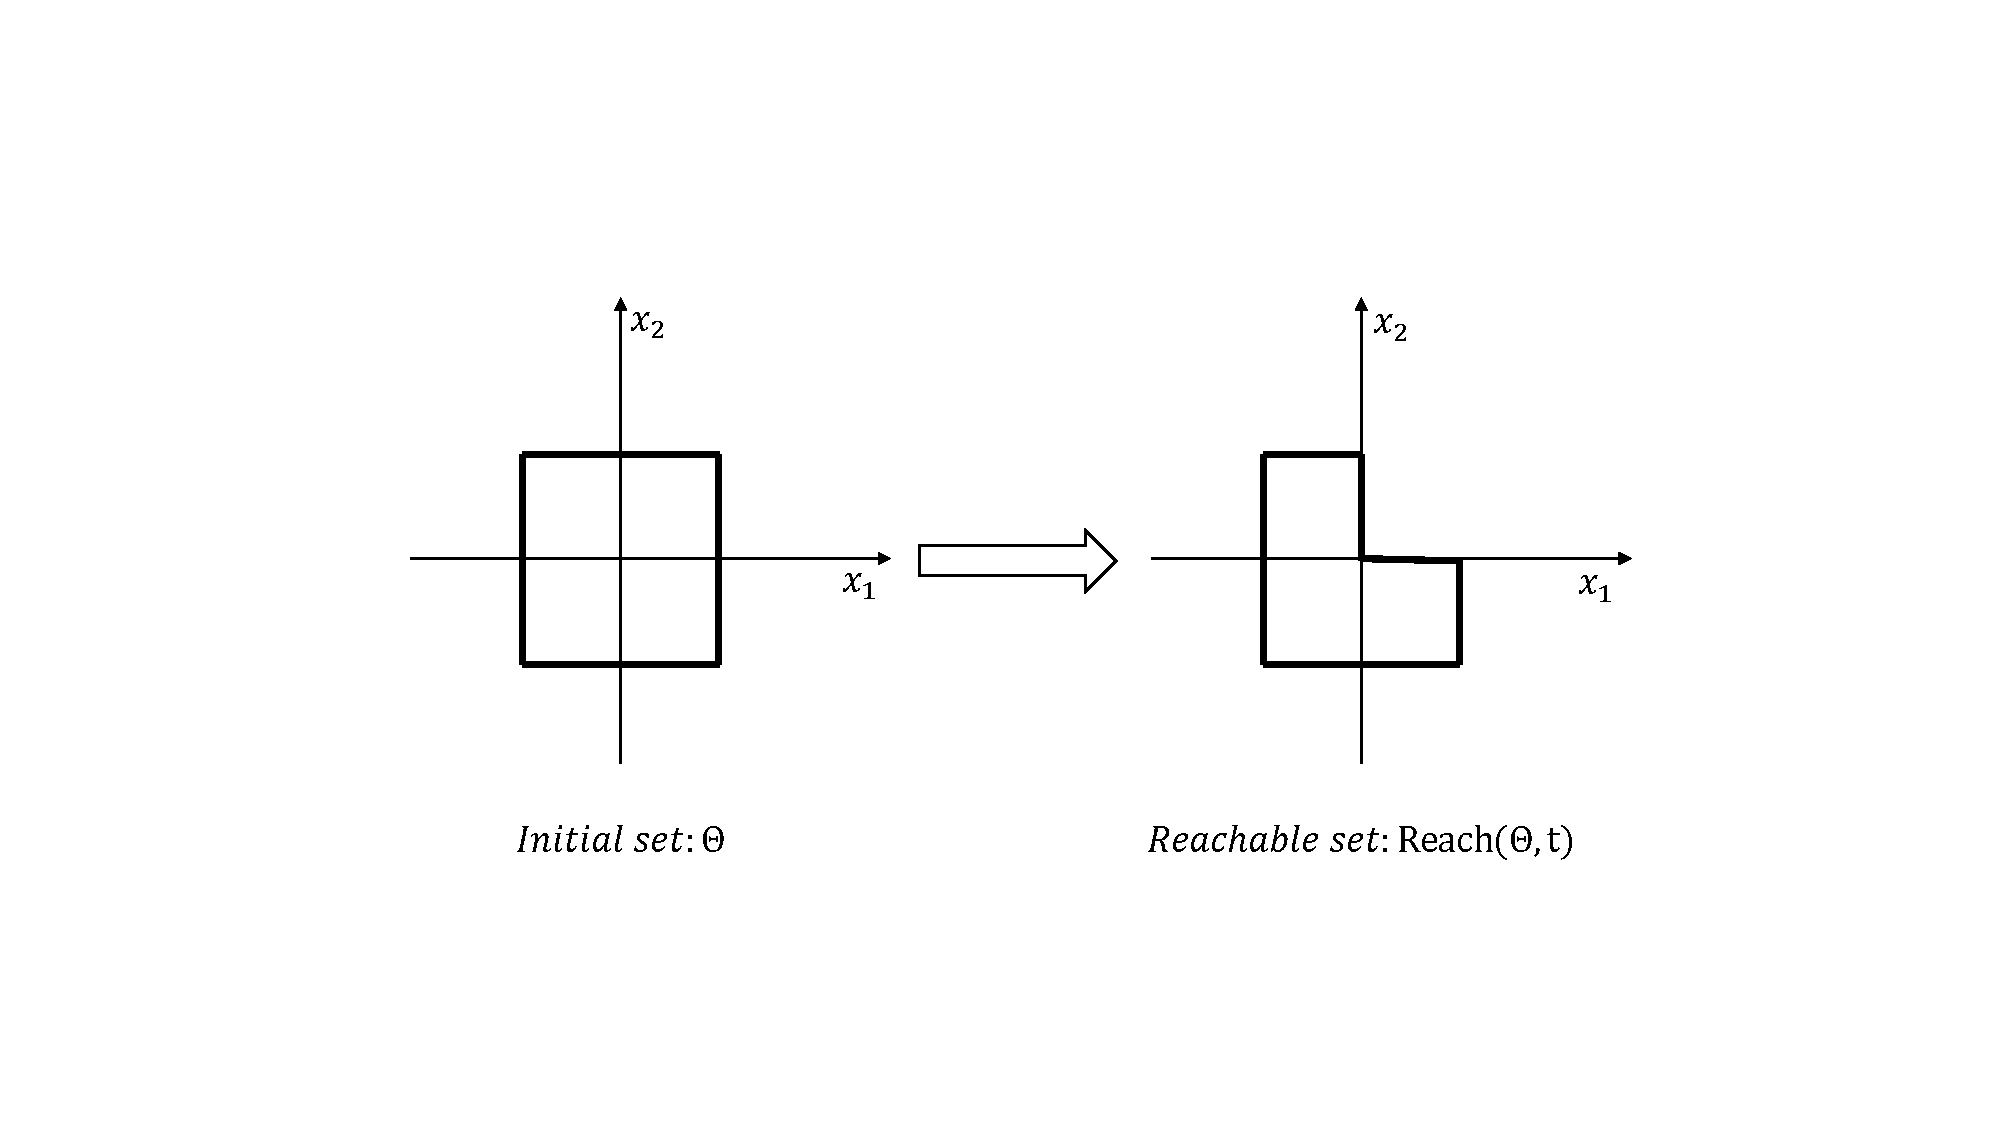
\includegraphics[width=12cm]{convex}
\caption{Starting from a convex set $\Theta$, $\reach{}(\Theta, t)$ is not convex}
\label{fig:convex}
\end{figure}

\end{enumerate}

\paragraph{Problem 2. (20 points)}
Show that a set of piece-wise continuous functions is closed under composition and linear combinations. That is, consider any two piece-wise continuous functions of time $f, g: \reals \rightarrow \reals^m$ with points of discontinuity ${\bf DC}_f$ and ${\bf DC}_g$. Show that
\begin{enumerate}[(a)]
\item $f \circ g$ is also piece-wise continuous.
\item For any $a_1, a_2 >0$, $a_1  f + a_2 g$ is also piece-wise continuous.
\end{enumerate}

\paragraph{Solution}
\begin{enumerate}[(a)]
% \item
% There is a counter-example. Let $g(x) = \begin{cases}
%       x \sin \frac{1}{x}, & \text{if}~x \neq 0\\
%       0, & \text{if}~x = 0\\
%     \end{cases}$ and ${\bf DC}_f = \{0\}$. Then we have $\forall x_i = \frac{1}{n\pi}, n = 1,2,3,\ldots$, $g(x_i) = 0$, and thus $f(g(x))$ is not continuous at $x_i$. Therefore in $[-1, 1]$, there exists infinitly many $x_i$ such that $f(g(x))$ is not continuous at $x_i$, which means $f \circ g$ is not a piecewise continuous function.
\item
$\forall x \not\in {\bf DC}_f \cup {\bf DC}_g$, $h = a_1  f + a_2 g$ is continuos at $x$. $\forall x \in {\bf DC}_f \cup {\bf DC}_g$ and $x \not\in {\bf DC}_f \cap {\bf DC}_g$, $h$ is not continuos at $x$. $\forall x \in {\bf DC}_f \cap {\bf DC}_g$, $h$ may be continuous or discontinuos at $x$. Therefore, ${\bf DC}_h \subset {\bf DC}_f \cup {\bf DC}_g$, which means $h$ has a finite number of points of discontinuity and is also piece-wise continuos.
\end{enumerate}

\paragraph{Problem 3. Billiards model (20 points)}
(a) Consider an idealized billiard table of length a and width b. The table has no pockets; its surface has no friction; and its boundary bounces the balls perfectly. Write a hybrid automaton model of the position of two balls of equal mass on this table. The balls have some initial velocities. A ball bounces off a wall when its position is at the boundary. Balls collide whenever $|x_1-x_2|\leq\varepsilon$ and $|y_1-y_2| \leq \varepsilon$ and their velocity vectors are pointing towards each other. Here $\varepsilon$ is some constant. Whenever a bounce occurs, the appropriate velocity changes sign. Whenever a collision occurs, the balls exchange their velocity vectors. Make all the variables internal. Wall bounces are modeled by an output action called bounce, and each collision is modeled by an output action collision.


(b) State and prove conservation of speed along each axis as an invariant property of the automaton.

\paragraph{Solution}
\begin{enumerate}[(a)]
\item
\noindent\rule{7cm}{1.0pt}\\
% \begin{lstlisting}[escapeinside={(*}{*)}]
\textbf{automaton} Billiards(a,b)\\
\tab\textbf{type}\\
\tab\textbf{actions}\\
\tab\tab bounce; collision;\\
\tab\textbf{variables}\\
\tab\tab $v_{1x}$:Real:=$v_{1x}^0$; $v_{1y}$:Real:=$v_{1y}^0$; $v_{2x}$:Real:=$v_{2x}^0$; $v_{2y}$:Real:$v_{2y}^0$; $x_1$:Real:=$x_1^0$; $y_1$:Real:=$y_1^0$; $x_2$:Real:$x_2^0$; $y_2$:Real:=$y_2^0$;\\
\tab\textbf{transitions}\\
\tab\tab bounce\\
\tab\tab \textbf{pre} $x_1 = 0 \vee x_1 = a$\\
\tab\tab \textbf{eff} $v_{1x} := -v_{1x}$;\\
\tab\tab bounce\\
\tab\tab \textbf{pre} $x_2 = 0 \vee x_2 = a$\\
\tab\tab \textbf{eff} $v_{2x} := -v_{2x}$;\\
\tab\tab bounce\\
\tab\tab \textbf{pre} $y_1 = 0 \vee y_1 = b$\\
\tab\tab \textbf{eff} $v_{1y} := -v_{1y}$;\\
\tab\tab bounce\\
\tab\tab \textbf{pre} $y_2 = 0 \vee y_2 = b$\\
\tab\tab \textbf{eff} $v_{2y} := -v_{2y}$;\\
\tab\tab collision\\
\tab\tab \textbf{pre} $|x_1-x_2| \leq \varepsilon \wedge |y_1-y_2| \leq \varepsilon \wedge (v_{1x}/v_{2x} = v_{1y}/v_{2y} < 0)$\\
\tab\tab \textbf{eff} $v_{1x} := v_{2x}$; $v_{2x} := v_{1x}$; $v_{1y} := v_{2y}$; $v_{2y} := v_{1y}$;\\
\tab\textbf{trajectories}\\
\tab\tab running\\
\tab\tab \textbf{evolve} $dx_1 = v_{1x}$; $dy_1 = v_{1y}$; $dx_2 = v_{2x}$; $dy_2 = v_{2y}$\\
\tab\tab \textbf{invariant} $(0<x_1<a) \wedge (0<y_1<b) \wedge (0<x_2<a) \wedge (0<y_2<b) \wedge (|x_1-x_2| > \varepsilon \vee |y_1-y_2| > \varepsilon \vee v_{1x}/v_{2x} \neq v_{1y}/v_{2y} \vee v_{1x}/v_{2x} \geq 0)$\\
%\end{lstlisting}
\noindent\rule{7cm}{1.0pt}

\item
$$I = \llbracket (|v_{1x}|+|v_{2x}| = |v_{1x}^0|+|v_{2x}^0|) \wedge (|v_{1y}|+|v_{2y}| = |v_{1y}^0|+|v_{2y}^0|) \rrbracket$$

\noindent (Start Condition) For the initial state, we have $|v_{1x}|+|v_{2x}| = |v_{1x}^0|+|v_{2x}^0|$ and $|v_{1y}|+|v_{2y}| = |v_{1y}^0|+|v_{2y}^0|$ according to the initialization statement in the model description.

\noindent (Transition Closure) After any ``bounce" action, the direction of the speed changes, but the absolute value of the speed doesn't change. Therefore, $\forall x \xrightarrow{\text{bounce}} x'$, if $x \in I$ then $x' \in I$. After the ``collision" action, $v_{1x}$ and $v_{2x}$ are exchanged, and $v_{1y}$ and $v_{2y}$ are exchanged. Thus if $|v_{1x}|+|v_{2x}| = |v_{1x}^0|+|v_{2x}^0|$ and $|v_{1y}|+|v_{2y}| = |v_{1y}^0|+|v_{2y}^0|$, then $|v_{1y}'|+|v_{2y}'| = |v_{1y}^0|+|v_{2y}^0|$ and $|v'_{1y}|+|v'_{2y}| = |v_{1y}^0|+|v_{2y}^0|$.

\noindent (Trajectory Closure) In the trjectory ``running" the speed variables never change, and thus $\forall \tau \in \mathbb{T}$, if $\tau$.fstate $\in I$, then $\tau$.lstate $\in I$.
\end{enumerate}

\paragraph{Problem 4. Hysteresis model (coding 40 points).}
(a) Model the following hysteresis-based switching system as a hybrid automaton. The automaton $\A$ has (at least) $n$ continuous variables $x_1,\ldots,x_n$ and a discrete variable called $m$ that takes the values in the set $m_1,\ldots, m_n$. For a state $\vx$ of the automaton, we say that the system is in $\mathit{mode}$ $m_i$, if $\vx \restr m =  m_i$. There are $n \times (n-1)$ actions $\auto{switch}(i,j)$, where $i, j \in [n]$ and $j\neq i$. When the system is in mode $m_i$,
\[
 \dot{x}_i=a_i x_i,
\]
where $a_i>0$ is a positive constant and $\dot{x}_j =0$ for all $j \neq i$. Further, when the system is in mode $m_i$, for any $j \neq  i$, if $x_i$ becomes greater than $(1+h)x_j$, then the automaton switches to mode $m_j$; otherwise, it continues in mode $m_i$. Here, $h > 0$ is a parameter of the model. Is your model deterministic?

(b) Write a simulator for this model and plot two executions starting from two different initial states: one where all the $x_i$'s are same, and another where they are different. For each execution, plot the duration that $\A$ stays in each mode. Can you conjecture something interesting about how long $\A$ stays in each mode?

\paragraph{Solution}
\begin{enumerate}[(a)]
\item
\noindent\rule{7cm}{1.0pt}\\
% \begin{lstlisting}[escapeinside={(*}{*)}]
\textbf{automaton} Switching(h)\\
\tab\textbf{type} Mode:enumeration [$m_1, \ldots, m_n$]\\
\tab\textbf{actions}\\
\tab\tab switch(i, j), for $i,j \in \{1,2,3,\ldots,n\}, i \neq j$\\
\tab\textbf{variables}\\
\tab\tab $m$:Mode; $x_i$:Real; for $i \in \{1,2,3,\ldots,n\}$\\
\tab\textbf{transitions}\\
\tab\tab switch(i, j), for $i,j \in \{1,2,3,\ldots,n\}, i \neq j$\\
\tab\tab \textbf{pre} $(m = m_i) \wedge (x_i > (1+h)x_j)$\\
\tab\tab \textbf{eff} $m := m_j$;\\
\tab\textbf{trajectories}\\
\tab\tab $Mode_i$ for $i \in \{1,2,3,\ldots,n\}$\\
\tab\tab \textbf{evolve} $dx_i = a_i x_i$;\\
\tab\tab \textbf{invariant} $(m = m_i) \wedge (x_i \leq (1+h)x_j)$ for $j \in \{1,2,3,\ldots,n\}, j \neq i$\\

%\end{lstlisting}
\noindent\rule{7cm}{1.0pt}

This model is nondeterministic. \textbf{pre} $(m = m_i) \wedge (x_i > (1+h)x_j)$ may be satisfied for more than one $j$ at the same time.

\item
Let $T_i$ be the total duration that the model stays in mode $i$. For every execution, we plot the variables $x_i$ as time grows. Some ececutions are plotted in Fig. \ref{fig:same}, Fig. \ref{fig:different} and Fig. \ref{fig:different_longer}.

After comparing the durations in Fig. \ref{fig:different} and Fig. \ref{fig:different_longer}, we can find that as the time $t$ goes to $\infty$, $\frac{T_i}{T_j}$ converges to $\frac{a_j}{a_i}$, i.e. $\lim_{t \to \infty} \frac{T_i}{T_j} = \frac{a_j}{a_i}$. We will give an informal proof in the following.

After every mode has been visited at least once, the following statement will hold: $x_{min} \leq x_i \leq x_{min}(1+h),~\forall i \in \{1,2,3,\ldots,n\}$, where $x_{min}$ is the minimal $x_i$ at this point of time. According to the dynamics of the model, we have $T_i = \frac{1}{a_i} \ln \frac{x_i}{x_i^0}$, where $x_i^0$ the initial value of $x_i$. Therefore, $\ln x_{min} - \ln{x_i^0} \leq a_i T_i \leq \ln x_{min} + \ln(1+h) - \ln{x_i^0}$. As $t$ goes to $\infty$, $x_{min}$ goes to $\infty$, and thus the inequation (or the interval) will be dominated by $\ln x_{min}$. Therefore, $\frac{a_i T_i}{a_j T_j}$ converges to 1, which implies $\lim_{t \to \infty} \frac{T_i}{T_j} = \frac{a_j}{a_i}$.
\end{enumerate}

\begin{figure}[h]
\centering
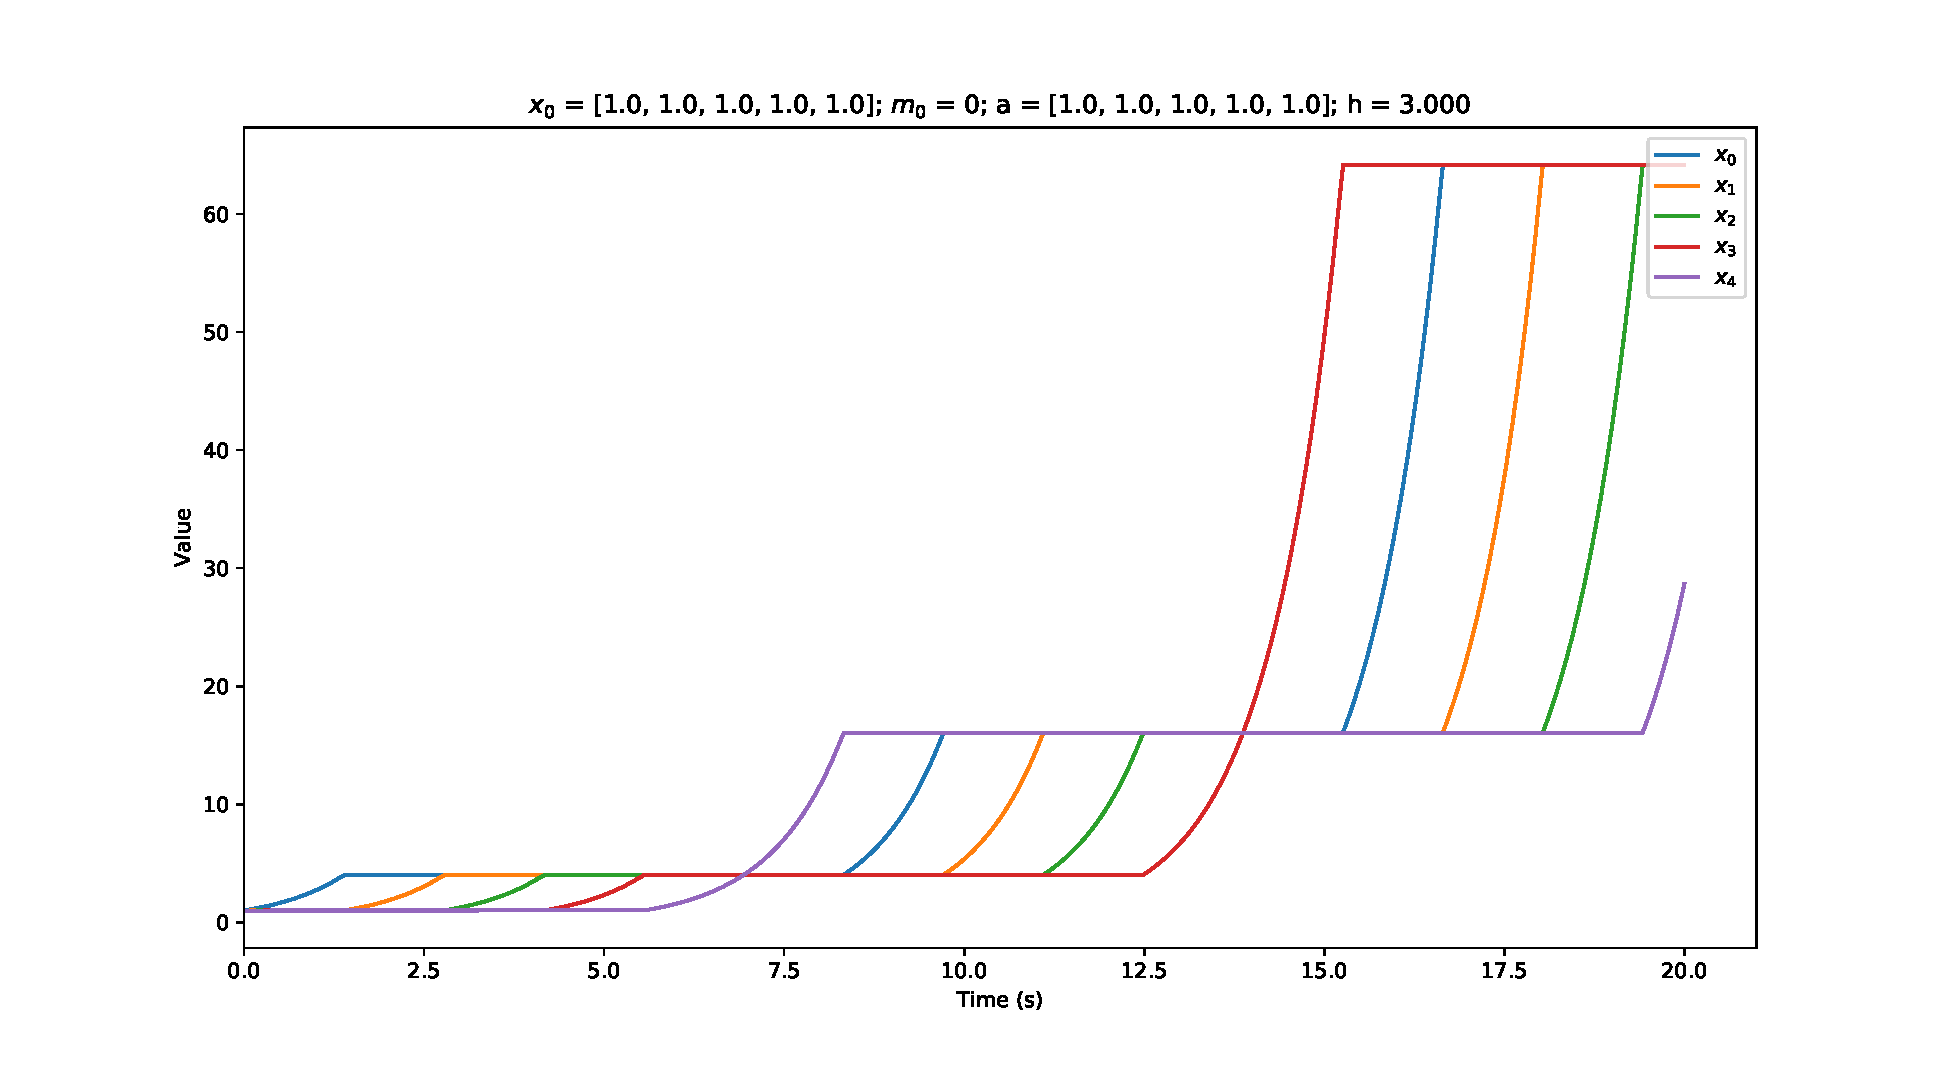
\includegraphics[width=12cm]{same_initial}
\caption{Starting from a state where all the $x_i$'s are same. The durations are [4.162, 4.161, 4.161, 4.161, 3.354].}
\label{fig:same}
\end{figure}

\begin{figure}[h]
\centering
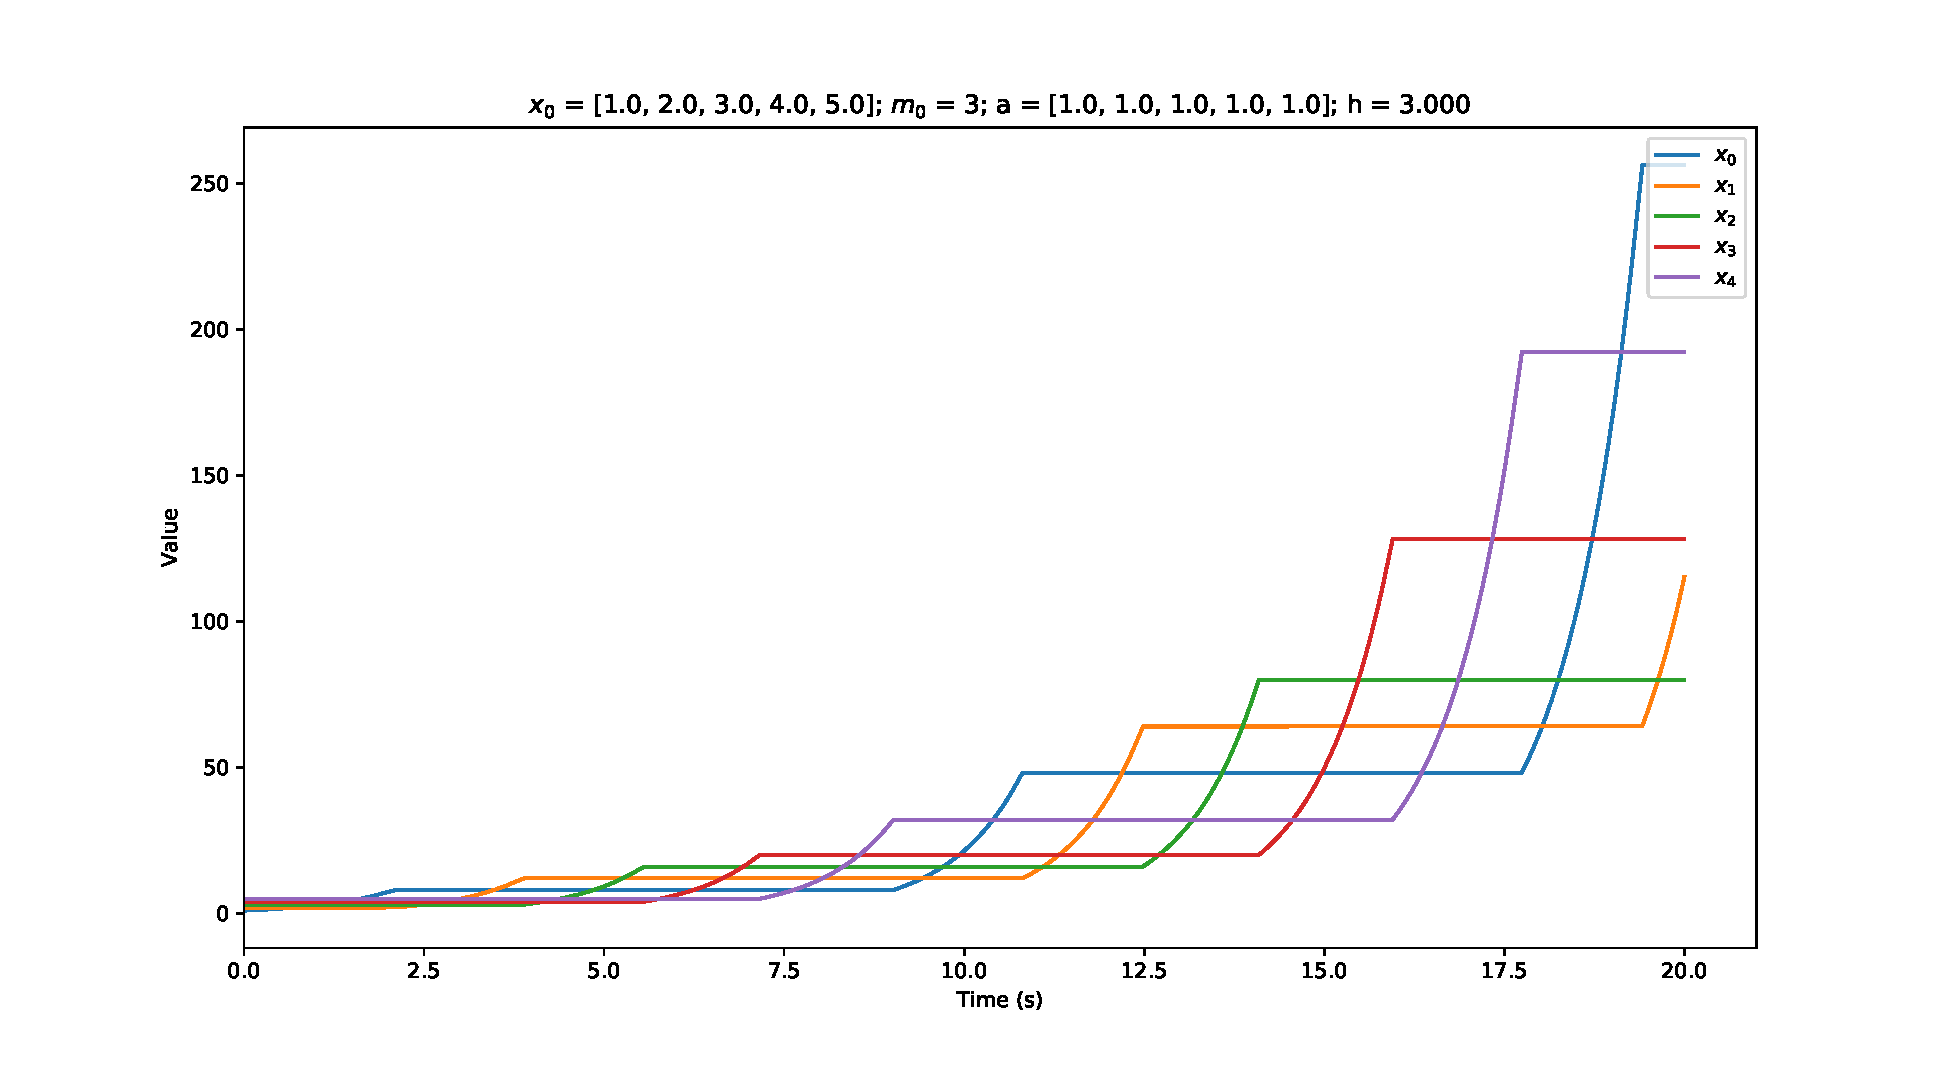
\includegraphics[width=12cm]{different_initial}
\caption{Starting from a state where $x_i$'s are different. The durations are [5.546, 4.052, 3.284, 3.468, 3.649].}
\label{fig:different}
\end{figure}

\begin{figure}[h]
\centering
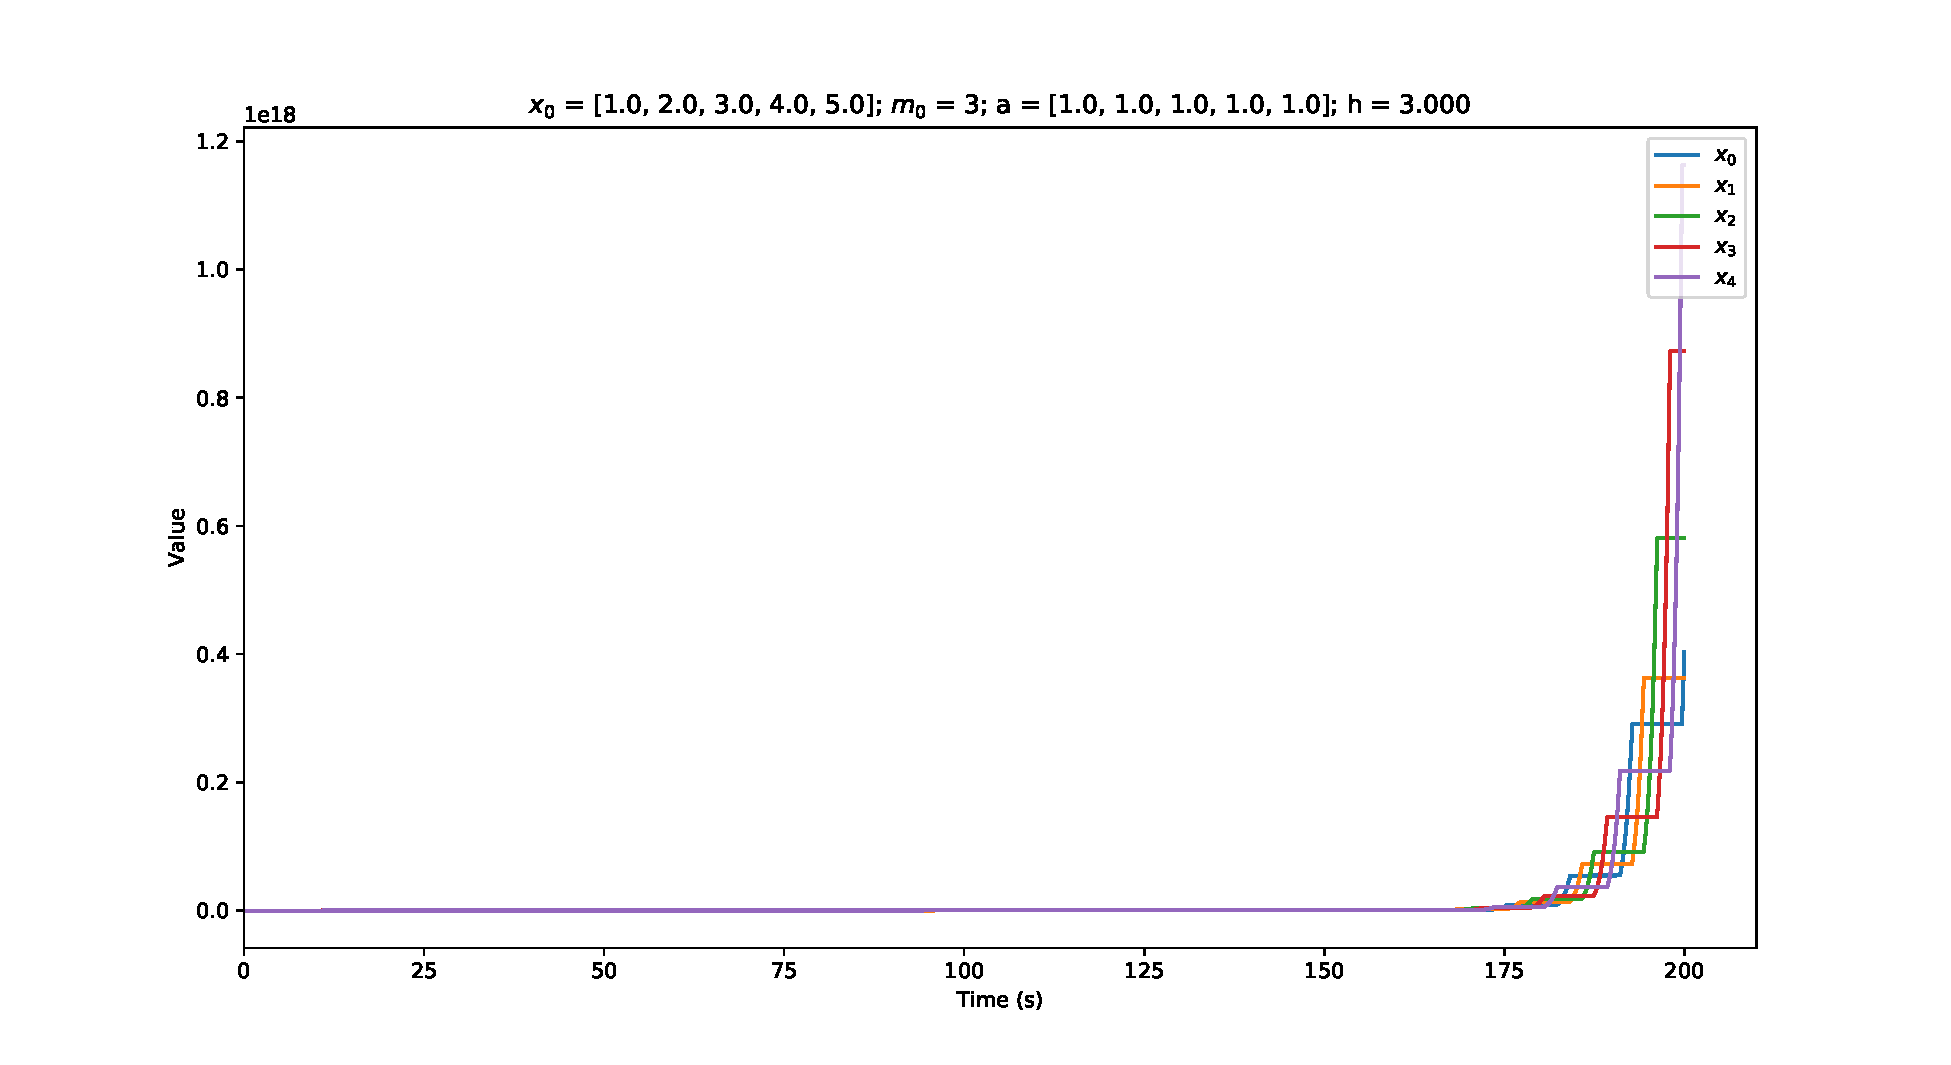
\includegraphics[width=12cm]{different_initial_longer}
\caption{Starting from a state where $x_i$'s are different (with a larger simulation budget). The durations are [40.539, 39.741, 39.806, 39.925, 39.988].}
\label{fig:different_longer}
\end{figure}

\paragraph{Class contribution and project ideas}
\begin{itemize}
\item Develop a simulator for the billiards example with multiple balls. Make it usable for others by paying attention to how the board, the initial positions and velocities of the balls are specified. Explicitly document how the collisions are detected in cases where multiple collisions may occur at the same time.
\item Develop a model and a simulator for Newton's cradle (search online).
\item Make your own  hybrid modeling problems and solutions. Lots of options here as almost everything can be modeled as a hybrid automaton: cars, drones, mixed-signal circuits, oscillators. Your problem should be (a) compact---describable in a couple of short paragraphs (e.g., like the billiards problem), (b) complete---fully specify the states, trajectories and transitions, and it has to be (c) interesting---the model should do something cool or showcase some property. You also need to provide the solution, of course.
\end{itemize}

%\bibliography{sayan1}
%	\bibliographystyle{plain}
\end{document}
